\documentclass[9pt, aspectratio=169]{beamer}

\usetheme{metropolis}
\setbeamertemplate{itemize items}{\faAngleRight}

\metroset{titleformat=smallcaps,block=fill,numbering=counter,progressbar=frametitle,sectionpage=none}
\setbeamersize{text margin left=5mm,text margin right=5mm} 
% %%%%%%%%%%%%%%%%%%%%%%%%%%%%%%%%%%%%%%%%%%%%%%%%%%%%%%%%%%%%%%%%%%%%%%%%%%%%%%
% \embedvideo{<poster or text>}{<video file (MP4+H264)>}
% \embedvideo*{...}{...}                     % auto-play
%%%%%%%%%%%%%%%%%%%%%%%%%%%%%%%%%%%%%%%%%%%%%%%%%%%%%%%%%%%%%%%%%%%%%%%%%%%%%%

\usepackage[bigfiles]{pdfbase}
\ExplSyntaxOn
\NewDocumentCommand\embedvideo{smm}{
  \group_begin:
  \leavevmode
  \tl_if_exist:cTF{file_\file_mdfive_hash:n{#3}}{
    \tl_set_eq:Nc\video{file_\file_mdfive_hash:n{#3}}
  }{
    \IfFileExists{#3}{}{\GenericError{}{File~`#3'~not~found}{}{}}
    \pbs_pdfobj:nnn{}{fstream}{{}{#3}}
    \pbs_pdfobj:nnn{}{dict}{
      /Type/Filespec/F~(#3)/UF~(#3)
      /EF~<</F~\pbs_pdflastobj:>>
    }
    \tl_set:Nx\video{\pbs_pdflastobj:}
    \tl_gset_eq:cN{file_\file_mdfive_hash:n{#3}}\video
  }
  %
  \pbs_pdfobj:nnn{}{dict}{
    /Type/RichMediaInstance/Subtype/Video
    /Asset~\video
    /Params~<</FlashVars (
      source=#3&
      skin=SkinOverAllNoFullNoCaption.swf&
      skinAutoHide=true&
      skinBackgroundColor=0x5F5F5F&
      skinBackgroundAlpha=0
    )>>
  }
  %
  \pbs_pdfobj:nnn{}{dict}{
    /Type/RichMediaConfiguration/Subtype/Video
    /Instances~[\pbs_pdflastobj:]
  }
  %
  \pbs_pdfobj:nnn{}{dict}{
    /Type/RichMediaContent
    /Assets~<<
      /Names~[(#3)~\video]
    >>
    /Configurations~[\pbs_pdflastobj:]
  }
  \tl_set:Nx\rmcontent{\pbs_pdflastobj:}
  %
  \pbs_pdfobj:nnn{}{dict}{
    /Activation~<<
      /Condition/\IfBooleanTF{#1}{PV}{XA}
      /Presentation~<</Style/Embedded>>
    >>
    /Deactivation~<</Condition/PI>>
  }
  %
  \hbox_set:Nn\l_tmpa_box{#2}
  \tl_set:Nx\l_box_wd_tl{\dim_use:N\box_wd:N\l_tmpa_box}
  \tl_set:Nx\l_box_ht_tl{\dim_use:N\box_ht:N\l_tmpa_box}
  \tl_set:Nx\l_box_dp_tl{\dim_use:N\box_dp:N\l_tmpa_box}
  \pbs_pdfxform:nnnnn{1}{1}{}{}{\l_tmpa_box}
  %
  \pbs_pdfannot:nnnn{\l_box_wd_tl}{\l_box_ht_tl}{\l_box_dp_tl}{
    /Subtype/RichMedia
    /BS~<</W~0/S/S>>
    /Contents~(embedded~video~file:#3)
    /NM~(rma:#3)
    /AP~<</N~\pbs_pdflastxform:>>
    /RichMediaSettings~\pbs_pdflastobj:
    /RichMediaContent~\rmcontent
  }
  \phantom{#2}
  \group_end:
}
\ExplSyntaxOff
%%%%%%%%%%%%%%%%%%%%%%%%%%%%%%%%%%%%%%%%%%%%%%%%%%%%%%%%%%%%%%%%%%%%%%%%%%%%%%

\usepackage{fontspec,minted}
\usepackage[scale=1]{ccicons}
\usepackage{metalogo}
\usepackage{xcolor,colortbl}
\usepackage{multicol,multirow,booktabs}
\usepackage{appendixnumberbeamer}
\usepackage{graphicx}
\usepackage{bm}
\usepackage{fontawesome}
\usepackage{csquotes}
\usepackage[backend=biber, natbib, sorting=nyt, doi=true, url=false, url=false, isbn=false, maxbibnames=10]{biblatex}
\addbibresource{../../utils/refs.bib}

\usepackage[spanish]{babel}
\usepackage{mathtools}
\usefonttheme{professionalfonts}
\usepackage{textcomp}

\setsansfont[BoldFont={Iwona Bold}, Numbers={Lining, Proportional}]{Iwona Light}
% \setmathsfont(Digits)[Numbers={Lining, Proportional}]{Fira Sans Light}
\setmonofont[Scale=MatchLowercase]{DejaVu Sans Mono}

\setbeamercolor{alerted text}{fg=red,bg=black!2}
\setbeamercolor{progress bar}{fg=red,bg=red!2}
\setbeamertemplate{itemize item}{\faCaretRight}
\setbeamertemplate{itemize subitem}{ \faAngleRight}
\setbeamertemplate{blocks}[shadow=false]
\setbeamercolor{block title}{bg=black!30,fg=red}
\setbeamercolor{block body}{bg=black!20,fg=black}
 
\usepackage{gensymb,amssymb}
\usepackage{upquote}
\usepackage{algpseudocode}
\algrenewcommand\algorithmicrequire{\textbf{Requiere}}
\algrenewcommand\algorithmicensure{\textbf{Devuelve}}
%\setbeamertemplate{blocks}[rounded][shadow=false]
\setbeamertemplate{blocks}[shadow=false]

\newcommand{\cx}{\column{0.5\textwidth}}
\newcommand{\cw}[1]{\column{#1\textwidth}}

\author{Manuel Carlevaro}
\date{{\tiny Departamento de Ingeniería Mecánica \\[-1em]
             Grupo de Materiales Granulares - UTN FRLP \\
        \faEnvelope{} manuel.carlevaro@gmail.com \- $\cdot$ \- \faTwitter{} @mcarlevaro}}
\institute{
  \vspace{6em}
  \centering
  {\tiny
  Cálculo Avanzado \enspace • \enspace 2022 \\
    \faLinux \- $\cdot$ \- \fontspec{TeX Gyre Pagella}\XeLaTeX \- $\cdot$ \- \ccbysa }
}

%% Operadores
\DeclareMathOperator{\sen}{sen}
\DeclareMathOperator{\sign}{sign}
\newcommand{\T}[1]{\underline{\bm{#1}}}
\DeclareMathOperator{\Tr}{Tr}

\usepackage{hyperref}
\hypersetup{
    colorlinks,
    citecolor=blue,
    filecolor=black,
    linkcolor=blue,
    urlcolor=blue
}
\urlstyle{same}

%% Códigos
\usepackage{minted}
\newminted[cpp]{cpp}{linenos,fontsize=\footnotesize,frame=lines,numbersep=4pt}
\newmintedfile[cppcode]{cpp}{linenos,fontsize=\footnotesize,frame=lines,numbersep=4pt}
\newcommand{\mic}[1]{\mintinline{C++}{#1}}

\newminted[py]{python}{linenos,fontsize=\footnotesize,frame=lines,numbersep=4pt}
\newminted[pyc]{pycon}{linenos,fontsize=\footnotesize,frame=lines,numbersep=4pt} % Consola de Python
\newminted[ipy3]{ipython3}{linenos,fontsize=\footnotesize,frame=lines,numbersep=4pt} % Consola de iPython3
\newmintedfile[pycode]{python}{linenos,fontsize=\footnotesize,frame=lines,numbersep=4pt}

\newmintedfile[makef]{basemake}{linenos,fontsize=\footnotesize,frame=lines,numbersep=4pt}
\definecolor{bg}{RGB}{22,43,58}
\newminted[shell]{console}{linenos=false,fontsize=\footnotesize,breaklines=true, frame=single} % Linea de comandos
\renewcommand\listingscaption{Código}

\makeatletter
\AtBeginEnvironment{minted}{\dontdofcolorbox}
\def\dontdofcolorbox{\renewcommand\fcolorbox[4][]{##4}}
\makeatother

% uso:
% Ejemplo de uso explícito:
% \begin{py}
% >>> list("abcd")
% ['a', 'b', 'c', 'd']
% \end{py}
% 
% Ahora ejemplo de código en file:
% \pycode{Chapters/intro/code/hola.py}
% 
% También se puede poner un sector del file:
% \pycode[firstline=6, lastline=7]{Chapters/intro/code/hola.py}
% 
% También se puede poner código \textit{inline}: \mip{print('¡Hola mundo!')} y en una sola línea:
% \slp|if __name__ == '__main__')|
% 
% Por último, se puede poner el código en un entorno \textit{float}, esto es, como las tablas y las figuras, con un caption y un label para luego hacer referencias, como por ejemplo al Código \ref{code:hola}.


\usepackage{tikz}
\usetikzlibrary{shapes,shadows,arrows,positioning,matrix,chains,backgrounds,fit}

\tikzset{
    %Define standard arrow tip
    >=stealth',
    %Define style for boxes
    obj/.style={
           rectangle,
           rounded corners,
           draw, very thick,
           text width=10em, fill=green!20,
           minimum height=2em,
           text centered, drop shadow},
    proc/.style={
	    rectangle, rounded corners,
	    draw,fill=red!50,very thick,
	    text width=8em,minimum height=2em,
	    text centered, drop shadow},
    % Define arrow style
    pil/.style={
           ->,
           thick,
           shorten <=2pt,
           shorten >=2pt,}
}

\setbeamertemplate{bibliography item}{%
  \ifboolexpr{ test {\ifentrytype{book}} or test {\ifentrytype{mvbook}}
    or test {\ifentrytype{collection}} or test {\ifentrytype{mvcollection}}
    or test {\ifentrytype{reference}} or test {\ifentrytype{mvreference}} }
    {\setbeamertemplate{bibliography item}{\faBook}}
    {\ifentrytype{online}
            {\setbeamertemplate{bibliography item}{\faGlobe}}
   {\setbeamertemplate{bibliography item}{\faFileText}}}%
  \usebeamertemplate{bibliography item}}

\defbibenvironment{bibliography}
  {\list{}
     {\settowidth{\labelwidth}{\usebeamertemplate{bibliography item}}%
      \setlength{\leftmargin}{\labelwidth}%
      \setlength{\labelsep}{\biblabelsep}%
      \addtolength{\leftmargin}{\labelsep}%
      \setlength{\itemsep}{\bibitemsep}%
      \setlength{\parsep}{\bibparsep}}}
  {\endlist}
  {\item}
\newcommand{\bcite}[1]{\citeauthor{#1}, \citetitle{#1} (\citeyear{#1})}


\title{Aproximación por mínimos cuadrados}
\subtitle{Motivación. Ajuste lineal. Ajuste polinómico. Ajustes potencial y exponencial.}

%%%%
% Bibliografía
%%%%

\begin{document}
\maketitle

\begin{frame}
\begin{columns}[t]
\cw{0.45}
\textbf{Datos:}

\begin{center}
\begin{tabular}{cccc}
\toprule
$x_i$ & $y_i$ & $x_i$ & $y_i$ \\
\midrule
 1 & 7.07 &  6 & 18.02 \\
 2 & 6.99 &  7 & 21.69 \\
 3 & 11.37 &  8 & 23.94 \\
 4 & 14.73 &  9 & 25.07 \\
 5 & 16.03 & 10 & 28.15 \\
\bottomrule
\end{tabular}
\end{center}

\cw{0.45}
\textbf{Figura:}
\begin{center}
    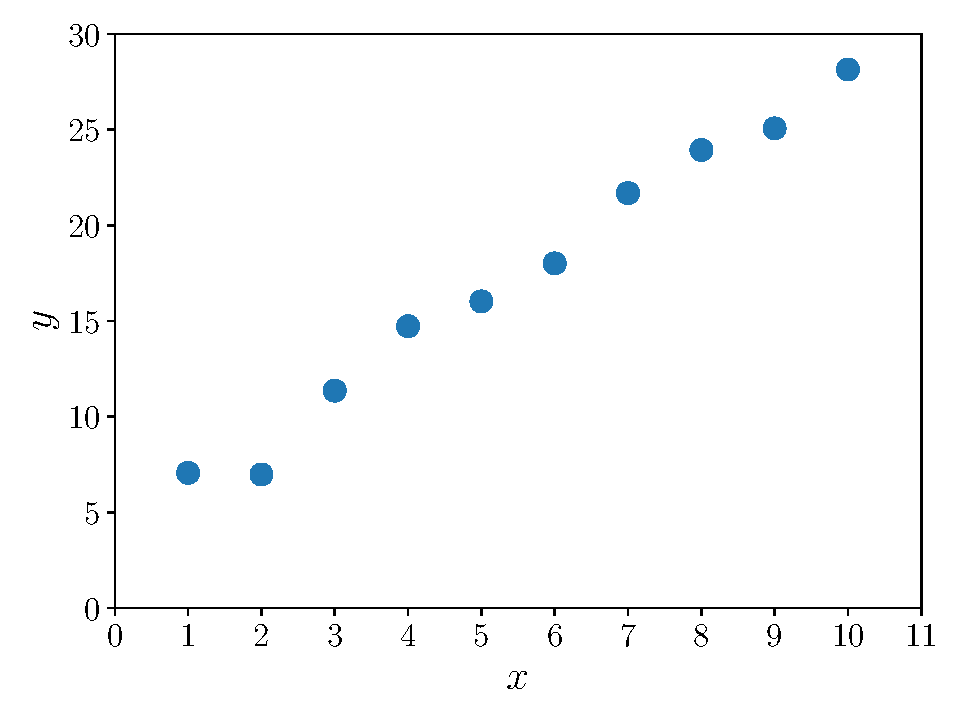
\includegraphics[scale=0.40]{figs/fig-01.pdf}
\end{center}
\end{columns}
\end{frame}

\begin{frame}
\begin{columns}[t]
\cw{0.45}
\textbf{Ajuste exacto:} polinomio de grado 9

\begin{align*}
    P_{9}(x) &= 30.63 - 55.47 x + 53.23 x^2 \\
             &- 30.82 x^3 \+ 12.24 x^4 -3.21 x^5 \\
             & +0.53 x^6 - 0.053 x^7 + 0.0029 x^8 \\
             &- 6.4 \times 10^{-5} x^9
\end{align*}
\begin{center}
    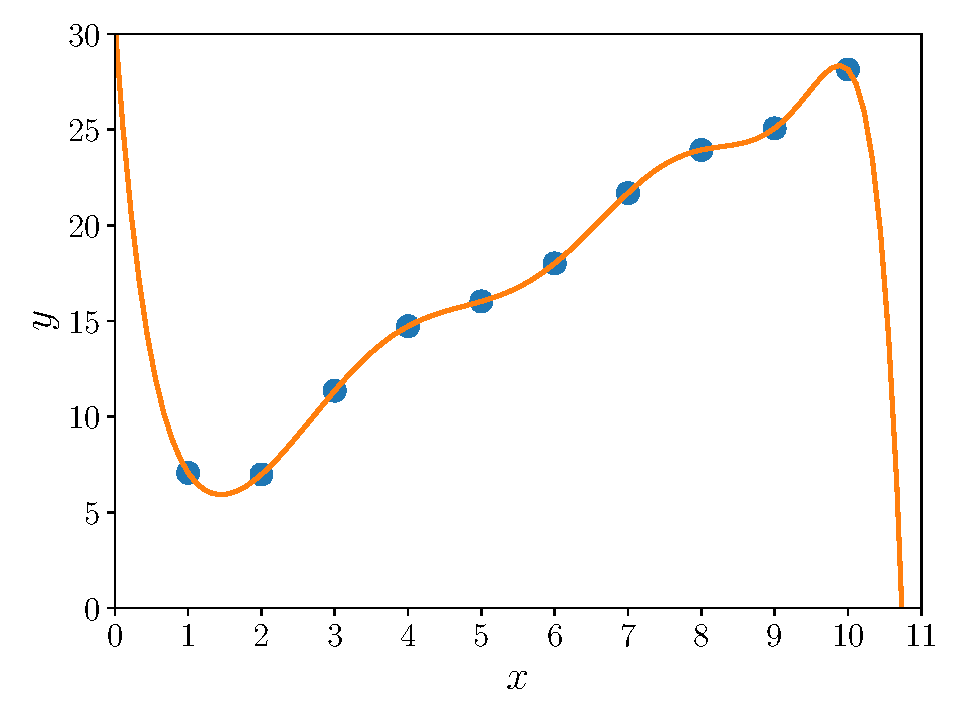
\includegraphics[scale=0.40]{figs/fig-02.pdf}
\end{center} \pause

\cw{0.45}
\textbf{Aproximación lineal:}
\[ y = a_1 \, x + a_0 \]

\begin{itemize}
    \item  Problema \textbf{minimax}: 
        \[ E_{\infty}(a_0, a_1) = \max_{1 \leq i \leq 10} \{|y_i - (a_1 x_i + a_0)|\} \]  \pause
    \item Desviación absoluta: 
        \[ E_1(a_0, a_1) = \sum_{i = 1}^{10} |y_i - (a_1 x_i + a_0) | \] \pause
    \item \textbf{Mínimos cuadrados:}
    \[ E_2(a_0, a_1) = \sum_{i = 1}^{10} [y_i - (a_1 x_i + a_0)]^2 \]
\end{itemize}
\end{columns}
\end{frame}

\begin{frame}
\begin{columns}[t]
\cw{0.55}
Para el conjunto $\{(x_i, y_i)\}_{i=1}^m$, \textbf{minimizar} respecto de \\ $a_0, a_1$:
\[ E \equiv E_2(a_0, a_1) = \sum_{i = 1}^{m} [y_i - (a_1 x_i + a_0)]^2 \] 
\pause
\[ \frac{\partial E}{\partial a_0} = 0 \txt{y} \frac{\partial E}{\partial a_1} = 0 \]
Esto es:
\[ 0 = \frac{\partial}{\partial a_0} \sum_{i = 1}^m [y_i - (a_1 x_i - a_0)]^2 = 2 \sum_{i=1}^m (y_i - a_1 x_i - a_o)(-1) \]
\[ 0 = \frac{\partial}{\partial a_1} \sum_{i = 1}^m [y_i - (a_1 x_i - a_0)]^2 = 2 \sum_{i=1}^m (y_i - a_1 x_i - a_o)(-x_i) \]
\pause

\cw{0.35}
\textbf{Ecuaciones normales:}
\begin{align*}
    a_0 \cdot m + a_1 \sum_{i=1}^m x_i &= \sum_{i=1}^m y_i \\
    a_0 \sum_{i=1}^m x_i + a_1 \sum_{i=1}^m x_i^2 &= \sum_{i=1}^m x_i \, y_i \\
\end{align*}
\pause

\textbf{Solución:}
\begin{align*}
    a_0 &= \frac{\dsum_{i=1}^m x_i^2 \dsum_{i=1}^m y_i - \dsum_{i=1}^m x_i y_i \dsum_{i=1}^m x_i}{m \left( \dsum_{i=1}^m x_i^2 \right) - \pow{\dsum_{i=1}^m x_i}{2} } \\
    a_1 &= \frac{ m \dsum_{i=1}^m x_i y_i - \dsum_{i=1}^m x_i \dsum_{i=1}^m y_i}{m \left( \dsum_{i=1}^m x_i^2 \right) - \pow{\dsum_{i=1}^m x_i}{2} } \\
\end{align*}

\end{columns}
\end{frame}

\begin{frame}
    \textbf{Ejemplo:} Encontrar la recta de mínimos cuadrados:
\begin{columns}
\cx
\begin{tabular}{ccccc}
\toprule
$x_i$ & $y_i$ & $x_i^2$ & $x_i y_i$ & $P(x_i) = 2.437 x_i + 3.903$ \\
\midrule
 1 & 7.07 &  1 & 7.07 & 6.34 \\ 
 2 & 6.99 &  4 & 13.97 & 8.78 \\ 
 3 & 11.37 &  9 & 34.10 & 11.21 \\ 
 4 & 14.73 & 16 & 58.92 & 13.65 \\ 
 5 & 16.03 & 25 & 80.14 & 16.09 \\ 
 6 & 18.02 & 36 & 108.10 & 18.52 \\ 
 7 & 21.69 & 49 & 151.85 & 20.96 \\ 
 8 & 23.94 & 64 & 191.52 & 23.40 \\ 
 9 & 25.07 & 81 & 225.62 & 25.83 \\ 
10 & 28.15 & 100 & 281.49 & 28.27 \\ 
\midrule
55 & 173.04 & 385 & 1152.77 & $E \approx 6.62$ \\
\bottomrule
\end{tabular}
\pause 

\cx
\begin{align*}
    a_0 &= \frac{385 (173.04) - 55 (1152.77)}{10 (385) - 55^2} = 3.903 \\
    a_1 &= \frac{10 (1152.77) - 55 (173.04)}{10 (385) - 55^2} = 2.437
\end{align*}

\begin{center}
    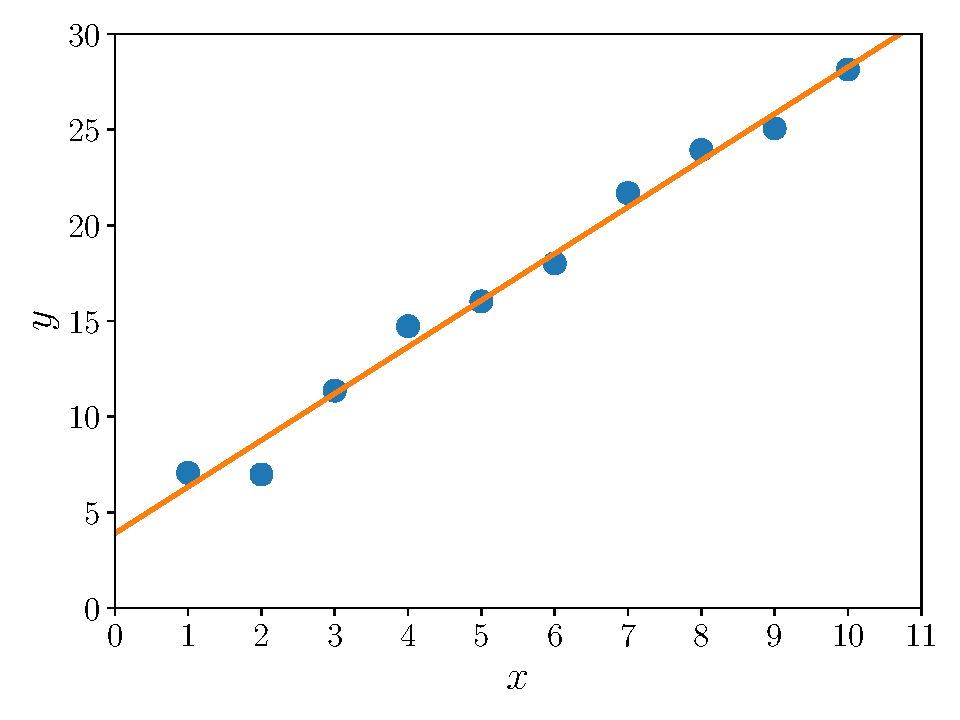
\includegraphics[scale=0.4]{figs/fig-03.pdf}
\end{center}
\end{columns}
\end{frame}

\begin{frame}
    \begin{columns}[t]
\cx
\textbf{Mínimos cuadrados polinomiales:}
\[ P_n(x) = a_n x^n + a_{n-1} x^{n-1} + \cdots + a_1 x + a_0 \]
$\{(x_i, y_i)\}, i = 1, \ldots m$, $n < m-1$. Minimizar:
\begin{align*}
    E &= \sum_{i=1}^m [y_i - P_n(x_i)]^2 \\
      &= \sum_{i=1}^m y_i^2 - 2 \sum_{i=1}^m P_n(x_i) y_i + \sum_{i=1}^m [P_n(x_i)]^2 \\
      &= \sum_{i=1}^m y_i^2 -2 \sum_{i=1}^m \left(\sum_{j=0}^n a_j x_i^j \right) y_i + \sum_{i=1}^m \pow{\sum_{j=0}^n a_j x_i^j}{2} \\
      &= \sum_{i=1}^m y_i^2 -2 \sum_{j=0}^n a_j \left( \sum_{i=1}^m y_i x_i^j \right) + \sum_{j=0}^n \sum_{k=0}^n a_j a_k \left( \sum_{i=1}^m x_i^{j+k} \right) 
\end{align*}
\pause

\cw{0.4}
Minimización: $\partial E / \partial a_j = 0, j = 0, 1, \ldots n$.
\[ 0 = \frac{\partial E}{\partial a_j} = -2 \sum_{i=1}^m y_i x_i^j + 2 \sum_{k=0}^na_k \sum_{i=1}^m x_i^{j+k} \]
$(n+1)$ \textbf{ecuaciones normales}:
\[ \sum_{k=0}^n a_k \sum_{i=1}^m x_i^{j+k} = \sum_{i=1}^m y_i x_i^j, \; j=0, 1, \ldots n \]
\end{columns}
\end{frame}

\begin{frame}
\begin{align*}
    a_0 \sum_{i=1}^m x_i^0 + a_1 \sum_{i=1}^m x_i^1 + a_2 \sum_{i=1}^m x_i^2 + \cdots + a_n \sum_{i=1}^m x_i^n &= \sum_{i=1}^m y_i x_i^0 \\ 
    a_0 \sum_{i=1}^m x_i^1 + a_1 \sum_{i=1}^m x_i^2 + a_2 \sum_{i=1}^m x_i^3 + \cdots + a_n \sum_{i=1}^m x_i^{n+1} &= \sum_{i=1}^m y_i x_i^1 \\
                                                                                                                     &\vdots \\
    a_0 \sum_{i=1}^m x_i^n + a_1 \sum_{i=1}^m x_i^{n+1} + a_2 \sum_{i=1}^m x_i^{n+2} + \cdots + a_n \sum_{i=1}^m x_i^{2n} &= \sum_{i=1}^m y_i x_i^n  
\end{align*}

\centering \alert{Solución única:} $x_i \neq x_j \quad \forall i \neq j$.
\end{frame}

\begin{frame}
\begin{columns}
\cx
    \textbf{Ejemplo:}
\begin{center}
\begin{tabular}{ccc}
    \toprule
    $i$ & $x_i$ & $y_i$ \\
    \midrule
    1 & 0 & 1.0000 \\
    2 & 0.25 & 1.2840 \\
    3 & 0.50 & 1.6487 \\
    4 & 0.75 & 2.1170 \\
    5 & 1.00 & 2.7183 \\
    \bottomrule
\end{tabular} 
\end{center} \pause

$n = 2, m = 5$
\begin{align*}
    5 a_0 + 2.5 a_1 + 1.875 a_2 &= 8.7680 \\
    2.5 a_0 + 1.875 a_1 + 1.5625 a_2 &= 5.4514 \\
    1.875 a_0 + 1.5625 a_1 + 1.3828 a_2 &= 4-4015
\end{align*} \pause

\textbf{Solución:}
\[a_0 = 1.005, \; a_1 = 0.8642, \; a_2 = 0.8437 \] 

\cx
\[P_2(x)= 1.005 + 0.8642 x + 0.8437 x^2 \]

\textbf{Error total:}
\[ E = \sum_{i=1}^5[y_i - P_2(x_i)]^2 = 2.74 \mul 10^{-4} \]
\pause

\begin{center}
    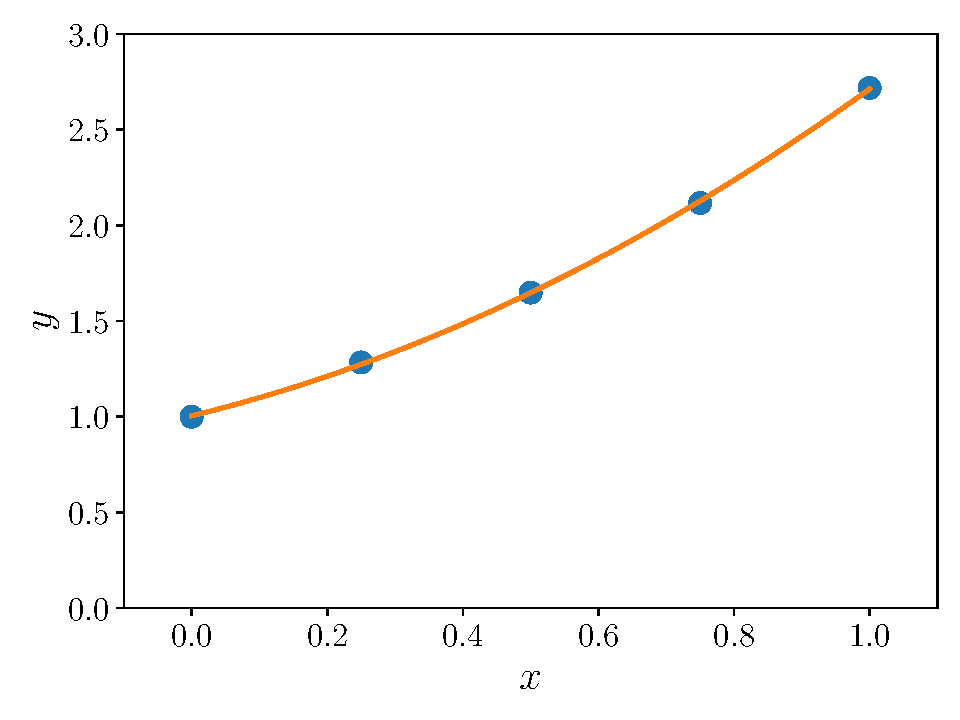
\includegraphics[scale=0.4]{figs/fig-04.pdf}
\end{center}

\end{columns}
\end{frame}


\begin{frame}
\begin{columns}[t]
\cx 
\textbf{Relación exponencial:}
\[ y = b \, e^{a x} \]
Minimizar:
\[ E = \sum_{i=1}^m (y_i - b e^{a x_i})^2 \]
Ecuaciones normales:
\begin{align*}
0 &= \frac{\partial E}{\partial b} = 2 \sum_{i=1}^m (y_i - b e^{a x_i})(-e^{a x_i}) \\
0 &= \frac{\partial E}{\partial a} = 2 \sum_{i=1}^m (y_i - b e^{a x_i})(-b x_i e^{a x_i}) \\
\end{align*}
\alert{Alternativa:}
\[ \ln y = \ln b + a x \]

\cx
\textbf{Relación potencial:}
\[ y = b \, x^{a} \]
Minimizar:
\[ E = \sum_{i=1}^m (y_i - b x_i^a)^2 \]
Ecuaciones normales:
\begin{align*}
0 &= \frac{\partial E}{\partial b} = 2 \sum_{i=1}^m (y_i - b x_i^{a})(-x_i^{a}) \\
0 &= \frac{\partial E}{\partial a} = 2 \sum_{i=1}^m (y_i - b x_i^{a})[-b \ln(x_i) x_i^{a}] \\
\end{align*}
\alert{Alternativa:}
\[ \ln y = \ln b + a \ln x \]
\end{columns}
\end{frame}


\begin{frame}
\begin{columns}
\cx
\textbf{Ejemplo:}

\begin{center}
\begin{tabular}{cccccc}
\toprule
$i$ & $x_i$ & $y_i$ & $\ln y_i$ & $x_i^2$ & $x_i \ln y_i$ \\
\midrule
 1 & 1.00 & 5.10 & 1.63 & 1.00 & 1.63 \\ 
 2 & 1.25 & 5.79 & 1.76 & 1.56 & 2.20 \\
 3 & 1.50 & 6.53 & 1.88 & 2.25 & 2.81 \\
 4 & 1.75 & 7.45 & 2.01 & 3.06 & 3.51 \\ 
 5 & 2.00 & 8.46 & 2.14 & 4.00 & 4.27 \\
\midrule
   & 7.50 & & 9.41 & 11.88 & 14.42 \\
\bottomrule
\end{tabular}
\end{center}

\cx
\begin{center}
    \begin{overprint}
    \onslide<1-2> 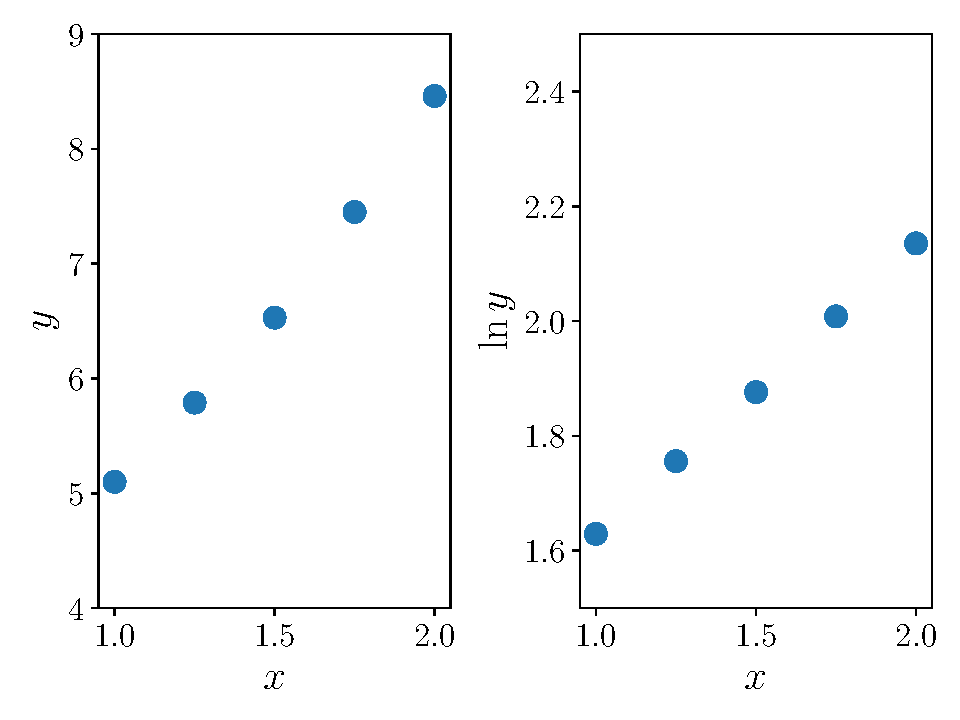
\includegraphics[scale=0.4]{figs/fig-05.pdf}
    \onslide<3> 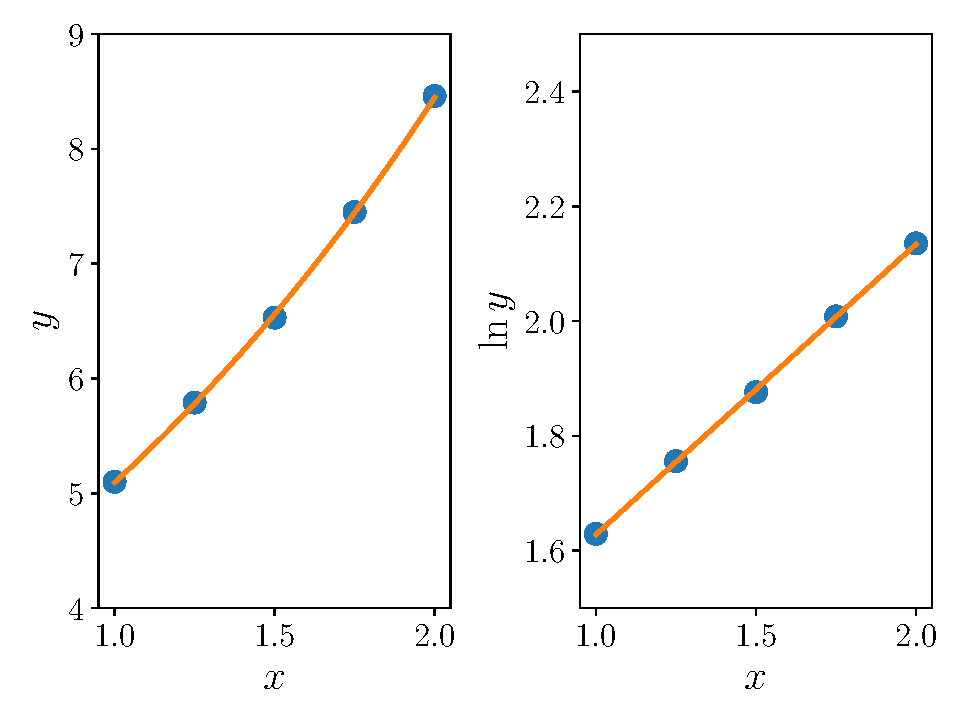
\includegraphics[scale=0.4]{figs/fig-05b.pdf} 
\end{overprint}
\end{center}
\end{columns} \pause

\begin{columns}
\cx
    \[ y = b e^{ax} \Rightarrow \ln y = \ln b + a x \]

\begin{align*}
    a &= \frac{5 (14.42) - (7.5)(9.41)}{5 (11.88) - (7.5)^2} = 0.5057 \\
    \ln b&= \frac{(11.88)(9.41) - (14.42)(7.5)}{5 (11.88) - (7.5)^2} = 1.122 
\end{align*}

\cx
$\ln b = 1.122 \rightarrow b = e^{1.122} = 3.071$
\[ y = 3.071 e^{0.5056 x} \]
\end{columns}
\end{frame}

\end{document}

